%%
%% This is file `sample-sigconf.tex',
%% generated with the docstrip utility.
%%
%% The original source files were:
%%
%% samples.dtx  (with options: `sigconf')
%% 
%% IMPORTANT NOTICE:
%% 
%% For the copyright see the source file.
%% 
%% Any modified versions of this file must be renamed
%% with new filenames distinct from sample-sigconf.tex.
%% 
%% For distribution of the original source see the terms
%% for copying and modification in the file samples.dtx.
%% 
%% This generated file may be distributed as long as the
%% original source files, as listed above, are part of the
%% same distribution. (The sources need not necessarily be
%% in the same archive or directory.)
%%
%%
%% Commands for TeXCount
%TC:macro \cite [option:text,text]
%TC:macro \citep [option:text,text]
%TC:macro \citet [option:text,text]
%TC:envir table 0 1
%TC:envir table* 0 1
%TC:envir tabular [ignore] word
%TC:envir displaymath 0 word
%TC:envir math 0 word
%TC:envir comment 0 0
%%
%%
%% The first command in your LaTeX source must be the \documentclass
%% command.
%%
%% For submission and review of your manuscript please change the
%% command to \documentclass[manuscript, screen, review]{acmart}.
%%
%% When submitting camera ready or to TAPS, please change the command
%% to \documentclass[sigconf]{acmart} or whichever template is required
%% for your publication.
%%
%%

\PassOptionsToPackage{table}{xcolor}
% \documentclass[sigconf]{acmart}
\documentclass[manuscript,screen,review]{acmart}


%%
%% \BibTeX command to typeset BibTeX logo in the docs
\AtBeginDocument{%
  \providecommand\BibTeX{{%
    Bib\TeX}}}

%% Rights management information.  This information is sent to you
%% when you complete the rights form.  These commands have SAMPLE
%% values in them; it is your responsibility as an author to replace
%% the commands and values with those provided to you when you
%% complete the rights form.
\setcopyright{acmcopyright}
\copyrightyear{2018}
\acmYear{2018}
\acmDOI{XXXXXXX.XXXXXXX}

%% These commands are for a PROCEEDINGS abstract or paper.
\acmConference[CHI '24]{Make sure to enter the correct
  conference title from your rights confirmation emai}{May 11--16,
  2024}{Honolulu, HI}
%%
%%  Uncomment \acmBooktitle if the title of the proceedings is different
%%  from ``Proceedings of ...''!
%%
%%\acmBooktitle{Woodstock '18: ACM Symposium on Neural Gaze Detection,
%%  June 03--05, 2018, Woodstock, NY}
\acmPrice{15.00}
\acmISBN{978-1-4503-XXXX-X/18/06}



%%
%% Submission ID.
%% Use this when submitting an article to a sponsored event. You'll
%% receive a unique submission ID from the organizers
%% of the event, and this ID should be used as the parameter to this command.
%%\acmSubmissionID{123-A56-BU3}

%%
%% For managing citations, it is recommended to use bibliography
%% files in BibTeX format.
%%
%% You can then either use BibTeX with the ACM-Reference-Format style,
%% or BibLaTeX with the acmnumeric or acmauthoryear sytles, that include
%% support for advanced citation of software artefact from the
%% biblatex-software package, also separately available on CTAN.
%%
%% Look at the sample-*-biblatex.tex files for templates showcasing
%% the biblatex styles.
%%

%%
%% The majority of ACM publications use numbered citations and
%% references.  The command \citestyle{authoryear} switches to the
%% "author year" style.
%%
%% If you are preparing content for an event
%% sponsored by ACM SIGGRAPH, you must use the "author year" style of
%% citations and references.
%% Uncommenting
%% the next command will enable that style.
%%\citestyle{acmauthoryear}

\usepackage{makecell}
\usepackage{multirow}

%%
%% end of the preamble, start of the body of the document source.
\begin{document}

%%
%% The "title" command has an optional parameter,
%% allowing the author to define a "short title" to be used in page headers.

% \usepackage{color, colortbl}
\definecolor{nsig}{rgb}{1,0.7,0.7}
\definecolor{sig}{rgb}{0.7,1,0.7}

% \title{Intentions are not defined by outcome alone! \\The case of inferring unrealised intentions by third-party intuition}
\title{The Discontent with Intent Estimation In-the-Wild: The Case for Unrealized Intentions}

%reframining intention estimation in terms of realised and unrealised intentions
%%
%% The "author" command and its associated commands are used to define
%% the authors and their affiliations.
%% Of note is the shared affiliation of the first two authors, and the
%% "authornote" and "authornotemark" commands
%% used to denote shared contribution to the research.
\author{Hayley Hung, Litian Li,  Jord Molhoek, and  Jing Zhou}

\email{h.hung@tudelft.nl}

% \authornotemark[1]
% \email{webmaster@marysville-ohio.com}
\affiliation{%
  \institution{Delft University of Technology}
  \country{The Netherlands}
}


% \author{Hayley Hung, Jord Molhoek, Litian Li, and  Jing Zhou}
% \email{h.hung@tudelft.nl}
% \affiliation{
%     \institution{Delft University of Technology}
%     \country{the Netherlands}
% }

% \author{Litian Li}
% \email{anon}
% \affiliation{
%     \institution{Delft University of Technology}
%     \country{the Netherlands}
% }

% \author{Jing Zhou}
% \email{anon}
% \affiliation{
%     \institution{Delft University of Technology}
%     \country{the Netherlands}
% }


% \author{Lars Th{\o}rv{\"a}ld}
% \affiliation{%
%   \institution{The Th{\o}rv{\"a}ld Group}
%   \streetaddress{1 Th{\o}rv{\"a}ld Circle}
%   \city{Hekla}
%   \country{Iceland}}
% \email{larst@affiliation.org}

% \author{Valerie B\'eranger}
% \affiliation{%
%   \institution{Inria Paris-Rocquencourt}
%   \city{Rocquencourt}
%   \country{France}
% }

% \author{Aparna Patel}
% \affiliation{%
%  \institution{Rajiv Gandhi University}
%  \streetaddress{Rono-Hills}
%  \city{Doimukh}
%  \state{Arunachal Pradesh}
%  \country{India}}

% \author{Huifen Chan}
% \affiliation{%
%   \institution{Tsinghua University}
%   \streetaddress{30 Shuangqing Rd}
%   \city{Haidian Qu}
%   \state{Beijing Shi}
%   \country{China}}

% \author{Charles Palmer}
% \affiliation{%
%   \institution{Palmer Research Laboratories}
%   \streetaddress{8600 Datapoint Drive}
%   \city{San Antonio}
%   \state{Texas}
%   \country{USA}
%   \postcode{78229}}
% \email{cpalmer@prl.com}

% \author{John Smith}
% \affiliation{%
%   \institution{The Th{\o}rv{\"a}ld Group}
%   \streetaddress{1 Th{\o}rv{\"a}ld Circle}
%   \city{Hekla}
%   \country{Iceland}}
% \email{jsmith@affiliation.org}

% \author{Julius P. Kumquat}
% \affiliation{%
%   \institution{The Kumquat Consortium}
%   \city{New York}
%   \country{USA}}
% \email{jpkumquat@consortium.net}

%%
%% By default, the full list of authors will be used in the page
%% headers. Often, this list is too long, and will overlap
%% other information printed in the page headers. This command allows
%% the author to define a more concise list
%% of authors' names for this purpose.
% \renewcommand{\shortauthors}{Hung et al.}
\renewcommand{\shortauthors}{Hung, Li, Molhoek and Zhou}

%%
%% The abstract is a short summary of the work to be presented in the
%% article.
\begin{abstract}
 % How often do we have an intention to do something that ends up not being realized? In HCI, we can register this as frustration. 
 
 The future of socially intelligent systems depends on developing abilities to anticipate and empathize with users. Whilst great strides have been made on developing systems for future behavior forecasting that sometimes also claim to do intention estimation, we argue that the predominant state-of-the-art treatment of these problems leads to a significant misunderstanding about this topic. This paper revisits intention estimation, describing the "intention by outcome" problem and how it severely limits a deeper understanding of the nature of the problem. We argue that without a deeper more nuanced understanding of how to develop intention estimation systems, we head into a severely biased world where intentions would only be considered valid by intelligent systems if they came true. Through a case study on estimating unrealized intentions to speak in-the-wild, we highlight open challenges of this largely unexplored topic.
\end{abstract}

%%
%% The code below is generated by the tool at http://dl.acm.org/ccs.cfm.
%% Please copy and paste the code instead of the example below.
%%
% \begin{CCSXML}
% <ccs2012>
%  <concept>
%   <concept_id>10010520.10010553.10010562</concept_id>
%   <concept_desc>Computer systems organization~Embedded systems</concept_desc>
%   <concept_significance>500</concept_significance>
%  </concept>
%  <concept>
%   <concept_id>10010520.10010575.10010755</concept_id>
%   <concept_desc>Computer systems organization~Redundancy</concept_desc>
%   <concept_significance>300</concept_significance>
%  </concept>
%  <concept>
%   <concept_id>10010520.10010553.10010554</concept_id>
%   <concept_desc>Computer systems organization~Robotics</concept_desc>
%   <concept_significance>100</concept_significance>
%  </concept>
%  <concept>
%   <concept_id>10003033.10003083.10003095</concept_id>
%   <concept_desc>Networks~Network reliability</concept_desc>
%   <concept_significance>100</concept_significance>
%  </concept>
% </ccs2012>
% \end{CCSXML}

% \ccsdesc[500]{Computer systems organization~Embedded systems}
% \ccsdesc[300]{Computer systems organization~Redundancy}
% \ccsdesc{Computer systems organization~Robotics}
% \ccsdesc[100]{Networks~Network reliability}

% \begin{CCSXML}
% <ccs2012>
%    <concept>
%        <concept_id>10003120.10003138.10003139.10010904</concept_id>
%        <concept_desc>Human-centered computing~Ubiquitous computing</concept_desc>
%        <concept_significance>500</concept_significance>
%        </concept>
   
%  </ccs2012>
% \end{CCSXML}

% \ccsdesc[500]{Human-centered computing~Ubiquitous computing}
%%
%% Keywords. The author(s) should pick words that accurately describe
%% the work being presented. Separate the keywords with commas.
\keywords{intention estimation, in the wild, speaking}
%% A "teaser" image appears between the author and affiliation
%% information and the body of the document, and typically spans the
%% page.
% \begin{teaserfigure}
%   \begin{tabular}{cc}
% 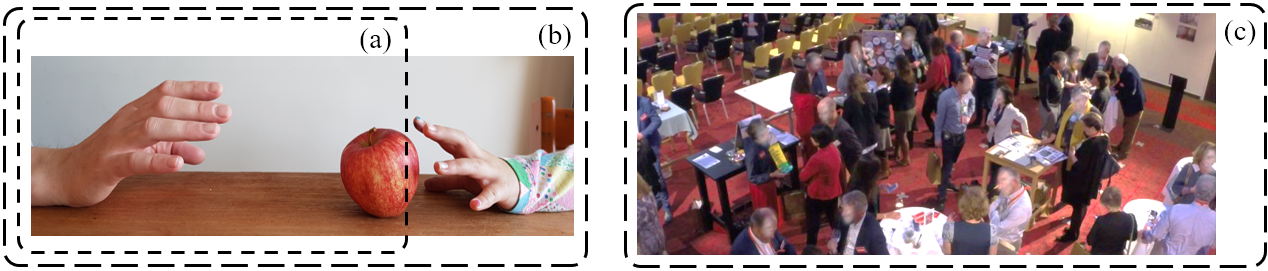
\includegraphics[width=0.66\textwidth]{samples/Teaser.png} & 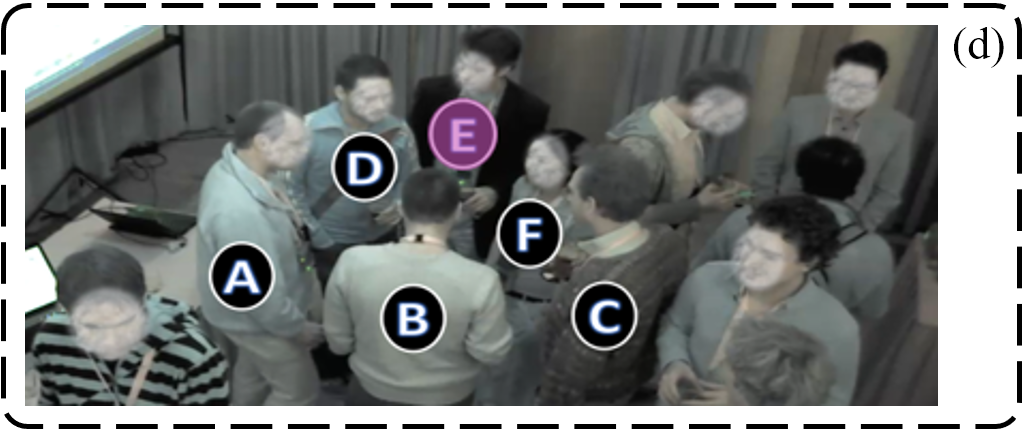
\includegraphics[width=0.33\textwidth]{samples/AnnotatedSocialStill.png}
%   \end{tabular}
%   \caption{Illustration of the intention by outcome problem. (a): Common setups involve an individual grabbing objects with gaze and posture. (b): When 2 or more people operate with competing goals, realized as well as unrealized intentions can occur. (c): Example of a crowded in-the-wild setting where people operate with hidden individual goals; coordinating to speak, leave, and join conversations emerge simultaneously with (un)realized intentions. (d) Does E intend to speak to D?}
%   \label{fig:teaser}
% \end{teaserfigure}
\begin{teaserfigure}
    \centering
  \begin{tabular}{cc}
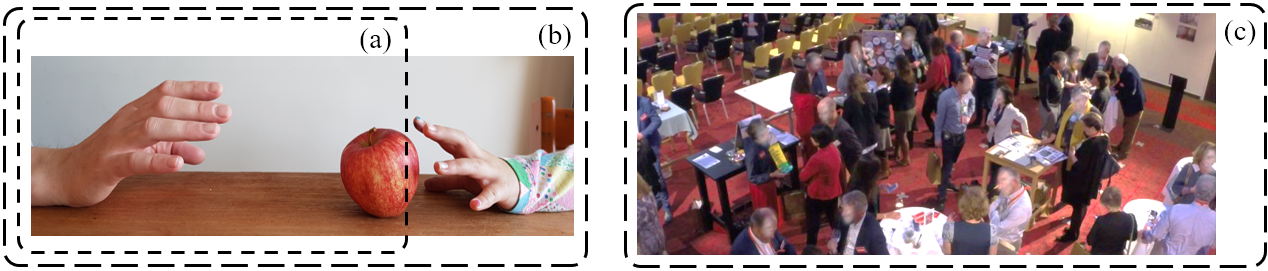
\includegraphics[width=0.87\textwidth]{samples/Teaser.png} & \\ 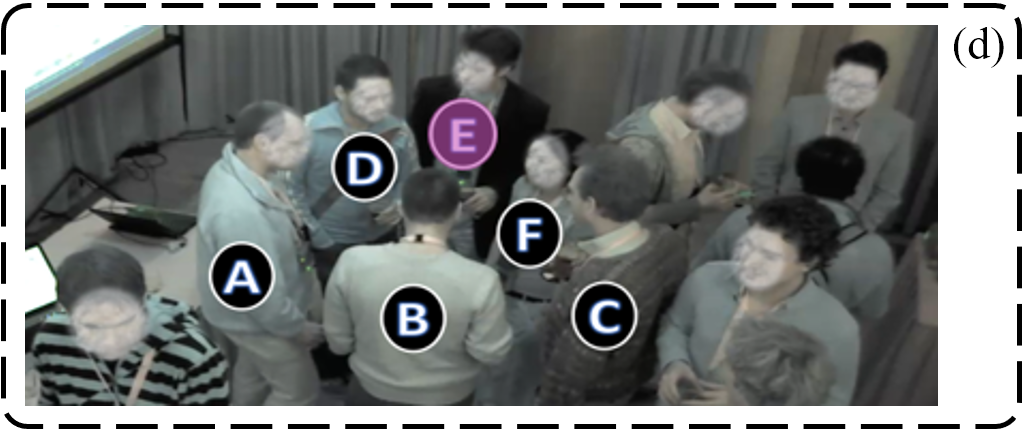
\includegraphics[width=0.43\textwidth]{samples/AnnotatedSocialStill.png}
  \end{tabular}
  \caption{Illustration of the intention by outcome problem. (a): Common setups involve an individual grabbing objects with gaze and posture. (b): When 2 or more people operate with competing goals, realized as well as unrealized intentions can occur. (c): Example of a crowded in-the-wild setting where people operate with hidden individual goals; coordinating to speak, leave, and join conversations emerge simultaneously with (un)realized intentions. (d) Does E intend to speak to D?}
  \label{fig:teaser}
\end{teaserfigure}

\received{20 February 2007}
\received[revised]{12 March 2009}
\received[accepted]{5 June 2009}

%%
%% This command processes the author and affiliation and title
%% information and builds the first part of the formatted document.
\maketitle

\section{Introduction}
% Effective multi-modal interaction relies on the ability to anticipate and empathize with humans. As a result, many researchers have investigated the problem of intention estimation \cite{Huang2015,Nie2021,CAO20171,objectpicking2021} and behavior forecasting \cite{ramansocproc2021,humantrajpredict2020}. One of the more popular approaches to designing and evaluating the effectiveness of intent prediction systems is using object picking tasks \cite{Huang2015,objectpicking2021,10.3389/fnbot.2021.647930}, which is very relevant in situations involving a human and an artificial agent who aims to serve the human, as illustrated in  Figure \ref{fig:teaser}(a). In general, approaches exploit behavioural cues such as gaze and posture to predict what the user intends to do next \cite{Huang2015,objectpicking2021,10.1007/s11263-018-1104-4}. The ground truth for the intentions are either pre-designed into the experiment\cite{10.1007/s11263-018-1104-4}, or it is assigned by observing a future outcome and labelling the past with the associated outcome \cite{objectpicking2021,Huang2015}. We call this the "intention by outcome" perspective, which leads to a heavy mischaracterization of the nature of the intention estimation. In non-competitive situations where the setting is designed primarily to facilitate the intention of a user, this is entirely appropriate. However in many more open ended settings such as Figure \ref{fig:teaser}(b) or (c), people are likely to be operating with hidden and potentially competing goals. 
This paper is about automated intention estimation. The goal of this paper is to highlight the challenges of developing intention estimation systems in Socially Intelligent Systems \cite{akata2020research,Vinciarellietalicv2009,picard2000affective}. For some readers this may be considered already as a very well trodden research task...perhaps even a solved problem! There is a lot of work already published in this field. For example, intention estimation has been investigated frequently in human robot interaction (e.g. object picking tasks \cite{Huang2015,objectpicking2021,10.1007/s11263-018-1104-4}, service robots \cite{ABBATE2024104568}), dialog systems where intent is typically one of the slots that need to be filled for understanding what action a user wants to do next, or what a user might be wanting to search for \cite{IntentMMSearch}. Those who have delved deeply into such a problem may also argue that the new name for intention estimation is behavior forecasting \cite{humantrajpredict2020,ramansocproc2021}. After all, a holy grail of intelligent systems are their ability to anticipate and respond to our needs. 

\subsection{Defining Intent}
Let's start with some formalities. Defining and understanding intention has been of interest in cognitive science and philosophy for a long time and remains a contemporary active field of study \cite{bratman1987intention,mele1992springs,plaks2015construal,doi:10.1080/09515089.2021.1915471}. In this paper, we take Bratman's \cite{bratman1987intention} definition of intentions by considering them as part of future action planning coupled with a belief by the individual that they have the ability to carry out the action. Crucially for intelligent systems, these planning behaviours need to be perceivable externally; what Mele in his book on understanding intentional behavior describes as \emph{overt intentional action} \cite{mele1992springs}. Crucially, Mele argued that there are two different types of intention; distal and proximal. The former describes a mental state related to the future which is not necessarily situated in the current situation. The latter refers to intentions related to immediate actions for which the closer we get to the action, the more likely it is that the behavior being observed is the action itself. One can easily get lost in the philosophical literature regarding intentions, intentionality and action. Fortunately, the survey of Bellardinelli provides a pragmatic balance for the interested reader \cite{belardinelli2023gazebased}. 

One final note on intention is its close relationship with action. As noted by Fuchs and Bellardinelli in the context of shared intention estimation in human-robot interaction \cite{10.3389/fnbot.2021.647930}, there is a blurred line between Where an intention stops and the intended action begins. However, what if the intended action never begins? Does that mean that the intention never existed? From the perspective of many existing research works on intention estimation. Intentions are operationalized in such a way that if it didn't happen, it wasn't intended to begin with. 

\subsection{The Forgotten Intention and the Intention by Outcome Problem}
We argue that this notion that something that doesn't happen was not intended in the first place is a major conceptual issue for Socially Intelligent Systems. As a side note, it when pitching this idea to Computer Scientists (CS) and Social Scientists (SS), there was a notable difference. The CS could not disentangle the difference between intentions and future behaviour whilst SS understood immediately the difference between intention, action, and outcome. It appeared that the CS were trapped in their own perspective bubble. 

We can summarize the problem with the state of the art understanding of intention estimation by observing Figure \ref{fig:teaser}(a). The classic trope for many intention estimation research works; a single hand reaches over the table, what will happen next? This is what the system typically sees at test time. However for the majority of research works on this topic, at data collection and training time, the development of ground truths for such settings is more complicated. Intentions can be enacted by asking subjects to perform a particular action which has been pre-determined and instructed to them \cite{10.1007/s11263-018-1104-4}, or the subject themselves decides on the outcome \cite{Huang2015}. The researcher then observes the recorded data and determines post-hoc what the intentions were by effectively looking into the future \cite{objectpicking2021,Huang2015}. At test time however, the system does not have the possiblity to observe the future. 

This paradigm of training pattern recognition and machine learning systems with more information at training time than is available at test time is a common technique which is used to ensure that good quality (potentially more objective) estimators are learned. However, this common practice shapes our perspective on how to design intention estimation systems. We call this \emph{"the intention by outcome"} problem.

The perspective shaping of former works channels our research activities into trying to transform intention estimation into an objective task when in reality intentions are conceptually not the same as future outcomes and have subjective and dynamic qualities. These simplifying assumptions made by prior work become the basis of how we understand the context of intention estimation, which we argue leads to the formation of a perspective bubble. Let's try to break that now. 

In each of these prior tasks, the user in those environments is the center of the world; systems are meant adapt to their needs. What if there are more users in these environments who are no longer interacting directly with an agent or interface but primarily with each other? A simple illustration of this point is seen in Figure \ref{fig:teaser} (b) where we see an expanded version of Figure \ref{fig:teaser}(a) to include a second hand on the right. Two hands reach over a table, what will happen next? The answer is that we do not know because we cannot predict the future. But we can make a good estimate. However, in this instantaneous moment, one would probably also not deny that both hands appear to indicate an intent to grab the apple.  

\subsection{From a Single User to a Constellation of Self-organizing Users}
The example of Figure \ref{fig:teaser}(b) gradually puts into focus how the context of use changes when building socially intelligent systems in more open-ended social situations like the social networking event show in Figure \ref{fig:teaser}(c). In these settings, socially intelligent systems are observing and interpreting the behaviours of multiple people with hopefully the capacity to help them. How would such a system understand that you are not having a good time at a party because you have not yet managed to escape a conversation and talk to the very interesting person you see across the room? Or that you still haven't managed to get a word in edge-ways with a particularly interesting conversation despite having some very interesting stories to tell? The major difference in such settings is that each individual in these scenes is no longer the center of a world where everything in the environment exists purely to satiate whatever immediate need or want that they have. When multiple people are involved, their needs and wants may vary and compete against each other.
% For instance, we know that even perceptions on when conversations should end vary greatly from one conversation partner to another [CITE conversation ending paper]

% Social well-being is listed in the constitution of the World Health Organization as a key factor of human health. On average, we spend 4-6 hours a day in face-to-face conversation \cite{Mehl2007} and we know of the physiological effects that positive social interactions can have on the body \cite{Heaphy2008}. Despite this we are missing key technologies that can help us to manage our social encounters more effectively e.g. a system that promotes inclusivity in professional networking by understanding if our social intentions were met.

Once we move away from the rather controlled settings of object picking tasks and a single user interacting with an application or an artificial agent (e.g. robot), the notion of unrealized intentions becomes a lot more apparent. Multiple humans engage in conversation and self-organize into an orderly system of cooperation to exchange information. How people coordinate themselves into conversations, especially as the complexity grows from a single meeting to a cocktail party or professional networking event remains an open field of study in Social Science \cite{KendonInteraction1990,dioszegietal2020b}. 

Once we move out of the lab and into more in-the-wild settings, we come against other problems. How can we read the mind of a person while they are the middle of a conversation? Won't they get distracted if they are asked to report on their intentions? Couldn't this contaminate their spontaneous overt intentional behavior? More will be elaborated on this point later in Section \ref{sec:challenge}.

\subsection{Who Cares About The Forgotten Intention? The Risks of the Intention by Outcome Problem}
While the earlier discussion highlights what may just be merely have been a slight conflation of conceptual terminology. We argue that scrutinizing a wider circle of potential applications of intelligent HCI systems, highlights significant challenges and also risks that must be overcome. This is because past work has only considered intention to be conceptualized as successful outcomes. 

Whilst there has been work to address how one might mitigate when `things don't work out' e.g. Frustration estimation in HRI settings \cite{10.3389/fpsyg.2021.640186}, there are many settings where unrealized intentions may occur frequently where multiple users need to coordinate with each other and simply minimizing frustration due to unrealized intentions might be unrealistic or just not the right way to approach the design of socially intelligent systems. After all, experiencing unrealized intentions may be an inevitable part of daily life. 

Helping users to navigate the complexities associated with living in real life may be more effectively approached if intelligent systems could understand or at least have a hypothesis about someone's mental state such as their intention. Note that this goes beyond being able to estimate someone's mood or emotions to being ultimately able to provide explanations for states of mind. e.g. "You appear frustrated. Is it because you wanted to join in on the conversation and didn't manage to?"

In the worst case ignoring unsuccessful intentions could pose a significant risk to the future development of intelligent systems and its potential risk of perpetuating the status quo rather than adapting to values of modern society such as efforts to reduce gender imbalance and reduce systematic racism. For example, it has been observed that female leaders emerge less frequently and appear to participate less in conversations \cite{badura2018gender,GERPOTT2018523,36a5eb2317d14d3aab58408b897ff673}. Working with an "intent by outcome" model of the world, this would mean that females do not speak up because they never intended to. In cases of criminal arrests, any racial minorities would be labelled as loitering with intent because they get arrested irrespective of whether they had negative intent or not. If we do not revisit the intention estimation problem, we continue to develop systems that discriminate and exclude.

\subsection{Relating Intentions and Outcomes: Predicting the Future is not the same as Intention Estimation}

Perhaps the mere notion of intentions are still hard to grasp. Let us use an example based on  social intentions in-the-wild as illustrated with Fig. \ref{fig:teaser} (d). We observe a conversing group containing participants A -- F at a professional networking event where F is speaking.  If we observe the gaze of E, we see that they are the only person not looking at F but is instead gazing at D. An observer might perceive this gaze to indicate an intention to talk to D. While state-of-the-art approaches would conclude that a system is successful in predicting E's intention if D and E start having a conversation. The main point here is that the perceived intention of E to speak to D is already observed and valid irrespective of whether D and E finally converse or not. 

\begin{figure}[tb]
    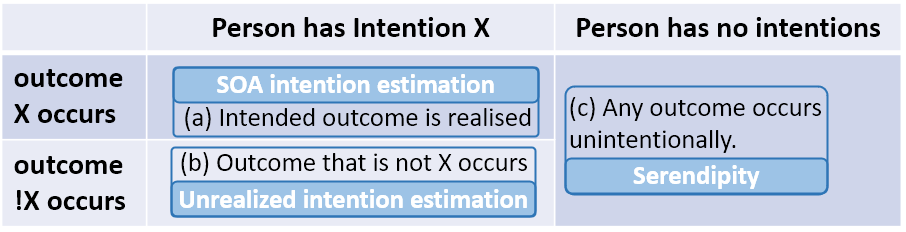
\includegraphics[width=\columnwidth]{samples/IntentQuad.png}
    \vspace{-5mm}
    \caption{Taxonomy of intentions: (a): realized intentions; (b): unrealized intentions; (c): serendipity}
    \vspace{-5mm}
    \label{fig:intent}
\end{figure}
There needs to be more attention on investigating automated means to estimate and distinguish between \emph{realized and unrealized intentions}. To do this more effectively it makes sense to think about the relationship between intentions and outcomes. Figure \ref{fig:intent} illustrates the possible combinations; state-of-art approaches focus on (a); realized intentions. These are intentions that led to the desired outcome. Meanwhile unrealized intentions (intentions that did not lead to the desired outcome), as shown in (b) have received only cursory attention \cite{wlodarczak2020breathing,Rasouli2019PIE}. For completeness we also include outcomes that can occur unintentionally, which can also be known as serendipity. For the simplicity of Figure \ref{fig:intent}, serendipity has been categorized to exist in settings where a person had no intention. A more nuanced definition of serendipity could define it actually as any unexpected outcome. In other words, an outcome could have occurred instead of an unrealized intention as well as an absence of intentions. When these potentially unrealized intentions are viewed from the lens of serendipity, it becomes again a hot topic in business \cite{Busch2020,Lane2021}, organizations \cite{eagle2004can,10.1145/2531602.2531641}, society \cite{Chan2019}, creativity and productivity \cite{gratton2020increase,meluso2020making} to name but a few. 

So why have unrealized intentions been of so little interest? Perhaps the focus of prior research work in intelligent systems were so focused on anticipating our intention in order to react to us, that it became synonymous with future forecasting. Or perhaps the problem is how do you identify and label something that was intended but did not happen?



\section{The Challenges of Unrealized Intention Labelling In-the-Wild}
\label{sec:challenge}
We hope that by now we have convinced the reader that intention estimation is an important and under-explored topic. Particularly in the case of unrealized intentions. So let's start to label them! The discerning reader may already see some hurdles ahead of us once we start to explore intentions in the absence of outcomes. How do we read the mind of the user? And how do we do it at fine time scales? When does an intention start and end? How do we label unrealized intentions both in terms of the relevant cues and also an outcome that \emph{did not occur?}. 

The challenges of labelling intentions can be illustrated in Fig. \ref{fig:selfvsthird}. For many, (including initially the authors themselves) self-report seems the only reasonable method to obtain labels of intentions. Ideally, the person would report constantly (\textbf{self-reported in-situ continuous feedback}: Fig. \ref{fig:selfvsthird}(a)), leading to a very temporally precise measure of someone's intention. Some tools have been developed to enable in-situ and in-the-wild reporting of affect whilst watching mobile video that may be applicable in this case \cite{zhang2020rcea}. However, this could disturb the spontaneity of the social behavior. Another alternative is to have subjects watch an interaction they just had and rate it continuously \cite{templeton2023long}. However this is hard to scale. Another solution involves individuals reporting their intentions just after finishing an interaction (\textbf{self-reported in-situ posthoc feedback}: Fig. \ref{fig:selfvsthird}(b)). However reflective cognitive processes can occur during post-hoc reflection leading to a difference in reported intention compared to a spontaneous in-situ report (see \cite{Dudzik2023} for a detailed discussion ). 
% Finally, whilst very powerful for artificial mind reading, self-report approaches for labelling intentions are hard to scale.
 
A final option uses external observers (\textbf{third-party continuous post-hoc feedback}: Fig. \ref{fig:selfvsthird} (c)). The temporal precision between the intention and sensor data is preserved, and the behaviour is not disturbed. However, whilst being much more scalable, it moves us further away from the truth of the individual being observed. There is perhaps still hope. While this may not be the same as the true intention of the person, learing plausible narratives of intention could still allow intelligent systems to reason about them, potentially updating and adjusting their understanding based on feedback during user interactions. Meanwhile the individual's true intentions are kept private. 
% other benefits including preserving the privacy of the subject until they want to reveal their true intention. However, in leveraging an annotator's own subjective life experiences, exploiting contextual knowledge from the setting will be important. However context estimation is another unsolved holy grail. 



\begin{figure}[tb]
    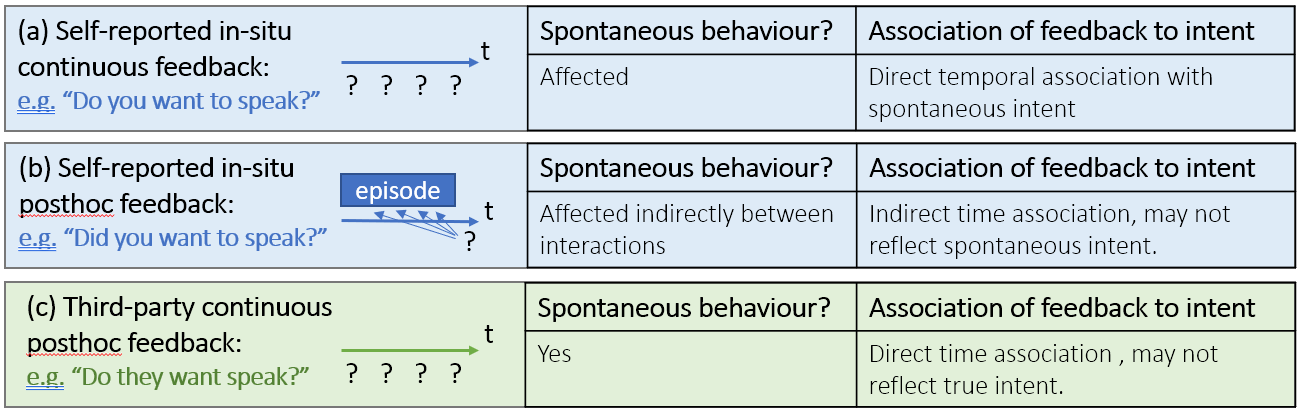
\includegraphics[width=\columnwidth]{samples/SelfvsThirdPartyIntentAnnotations_v3.png}
        \vspace{-5mm}
    \caption{Challenges to overcome for labelling realized and unrealized intentions. We present a study using (c) in Sec. \ref{sec:case}.}
        \vspace{-5mm}
    \label{fig:selfvsthird}
\end{figure}

\subsection{Gut Reactions and Cognitive Empathy}
It would appear that exploiting the perceptions of external observers would be a nice compromise for obtaining intentions at scale and with high temporal fidelity. But what makes this approach valid? By asking annotators to label plausible intentions, they are likely to simulate narratives plausible to their own life experiences \cite{Decety2004,barrett2017emotions,Ridderinkhof2022}. On the other hand, given that the individual being observed is not the same as the observer, there is some distance that must be taken by an observer. 

One can also consider such labelling tasks to be a form of Ethnomethodology, which is deliberately agnostic towards social theory in favour of a naiive eye, shaped towards the context of interest. This is an important notion as ``..members of society must have some shared methods that they use to mutually construct the meaningful orderliness of social situations” \cite{Blackwell2003}. Stated another way, the basic premise of Ethnomethodology assume that there is an emergent and meaningful orderliness to social situations that can be interpreted by external observers. 

In the end it is likely that observers, and in particular lay observers if we take a crowd sourcing approach to the labelling process, will not necessarily be trained in the rigours of Ethnomethodological practice. And even if they were, disentangling the effect of subjective personal experience from a deliberate naiive eye approach may be impossible. 

What is clear, however, is that these perceived intentions come with plausible narratives or explanations. It could well be that for a given constellation of behaviours, much like those seen in Figure \ref{fig:teaser}(d), multiple plausible explanations for completely different perceived intentions for person E could exist. In the crowdsourcing literature, there has been a tendency to assume one single ground truth. Annotations are judged as being poor if they do not agree with other annotators and there are some people who are more expert than others\cite{10.1609/aimag.v36i1.2564}. 

Finally what happens in the case of unrealized intentions? We propose that gut instincts may be the way to identify them and in the following case study, we investigate this approach to label unrealized intentions to speak.

% \subsection{From Whom and When is the Intention Inference Obtained?}
% explanation of multiple interpretations of an individual's intent (their own, external observer)

% \subsection{Who's intent inference should we be learning from?}
% \begin{itemize}
%     \item discussion of validity of individual's self reported intention (during and posthoc)
%     \item discussion of validity of external observation of intention 
% \end{itemize}

% \subsection{Where can Intention Perceptions exist?}
% In constructing this explanation of the apparent intention, in Figure \ref{fig:teaser}, the user is at the center of the scene. The assumption is that intelligent systems must necessarily read the mind of the user in order to fulfil their every need. If we take a more pervasive or ubiquitous view on intelligent systems, we can expand the focus of potential inference to the understanding of one of many users embedded in a intelligent environment where multiple perspectives of intention can exist. There is (i) the true intention of a given person in the scene, (ii) their perception of their own intention, (iii) their intention as perceived by other interlocutors who might have their own stakes in a particular interaction, and (iv) their intention as perceived by an external observer who has no interdependent relationship with anyone in the scene. Highlighting these 4 perspectives also showcases that for a given situation and behaviour, 





% \begin{itemize}
%     \item why are unrealised intentions important to capture
%     \item what are we actually doing these days?
%     \item what make capturing unrealised intentions hard challenges of doing this in the wild (no standardised way of thinking about this, are realised and unrealise intentions observable in the same way? issues of semantics and resolution of that forces us to think more deeply about the truth we are searching for. 
% \item show that we cannot easily ask people whilst making it scalable
% still the issue of label sparsity as we may still miss quite a few observations. 
% \item Need datasets able to capture high quality audio as well as video so that we can characterise this. is this something that can be crowdsourced? 
% \item challenges of label noise, 
% \item need for some form of super annotator that is sensitive to these issues? Seeing things that no one else sees.
% A form of artificial empathy?
% \item First person or third party perceptions. ....The validity of truth.

% \end{itemize}
% Ethics of machines that can do it, ethics of machines that cannot do it?









% \noindent
% \subsubsection*{Main stream machine perception avoids cognitive modelling in machine perception tasks}
% % \vspace{-2mm}

% % Whilst there have been some great efforts to model intention in the HRI and HCI community, 

% \noindent
% Whilst this paper makes an argument for unrealized intention estimation, this particular usecase serves to highlight a major conceptual challenge we still face when injecting In other related mainstream computer science fields such as Computer Vision and Pattern Recognition, Su and Crandell highlight an important gap in the field observing that the community has shifted away from " [explaining] the internal cognition of people...[to] merely [describing] the external behavior of people" \cite{AffectiveGrowthCV2021}.




\section{Case Study: Estimating Unrealized Intentions to Speak} \label{sec:case}
As highlighted in Sec. \ref{sec:challenge}, there are compelling benefits to using third party labels. To this end, we present a case study that investigates the estimation of proximal intentions. We focus specifically on two questions, focusing on the problem of speaking intention in-the-wild: (i) How feasible is it to label unrealized intentions using an external observer? Can we rely on Mele's idea of overt intentional actions\cite{mele1992springs}? (ii) How could we train a model to detect realized and unrealized intentions? (iii) would there be a difference between the performance of realized and unrealized intentions?
% This allows us to investigate how realized and unrealized intentions may be related and the challenges of doing this in a in-the-wild ecologically valid setting. 
% Second, we focus on the modality of body worn acceleration although the same setting could be extended to a multi-modal setup. 
\subsection{Related Work on Intentions to Speak}
To our knowledge, Wlodarczak and Heldner carried out the only research that has discussed unrealized intentions to speak \cite{wlodarczak2020breathing}. They used sensors strapped to the chest and abdomen in seated discussions to measure breathing during conversations. The findings identified breath inhalations (that looked like preparations to speak) followed by long breath holds and a silent exhalation with no accompanying speech activity. They speculated that this behaviour could be indicative of unrealized intentions. Their findings are foundational but their sensing approach is hard to scale to dynamic in-the-wild ecologically valid settings. Moreover, their speculations were not validated with self-reports or third-party perceptions of the multi-modal data. 

Other related work focuses mainly on behaviour forecasting, namely turn-change prediction and next-speaker prediction. Turn-change prediction estimates \emph{when} a turn change is about to occur whilst next-speaker prediction estimates \emph{who} will speak next. Petukhova and Bunt \cite{whosnext} found that gaze aversions, lip movements, and posture shifts are strongly correlated with receiving the next turn in conversations. According to Novick et al., 42\% of the turn changes follow the pattern: the speaker first looks towards the listener as they complete the turn; then the speaker and the listener have a short moment of eye contact; lastly the listener looks away and begins speaking \cite{novick_gaze}. Automatic recognition of such patterns can be useful for next speaker prediction and possibly for prediction of intentions to speak. As noted by Schegloff, turn-taking is not always smooth, as an interruption could be interpreted as not letting the current speaker finish, which can be viewed conceptually as a form of unrealized intention \cite{schegloff2001accounts}.

Ishii et al. showed that gaze-transition patterns are useful for predicting the next speaker and when the next speaker starts to speak. They later found that a fusion model using both respiration and gaze behaviour performs better than using only one of them in isolation, and respiration was the more useful feature in their multimodal model \cite{ishii2015multimodal}. A followup study also by Ishii et al. found that people tend to open their mouths slightly before they start speaking, which can be related to intentions to speak \cite{mouth_open_patterns}. 

% not in the wild
% Several studies have mentioned using multi-modalities 
% Several studies have found some related social cues and behavioral patterns of turn-changing in the conversations. The work of Petukhova and Brunt \cite{whosnext} found gaze aversions, lip movements and posture shifts are strongly correlated with receiving the next turn in conversations. According to Novick et al., 42\% of the turn changes follow the pattern: the speaker first looks towards the listener as they complete the turn; then the speaker and the listener have a short moment of eye contact; lastly the listener looks away and begins speaking \cite{novick_gaze}. Automatic recognition of such patterns can be useful for next speaker prediction and possibly for prediction of intentions to speak. In a multi-party conversation, turn-taking can also become rigid sometimes, as an interruption, which can be interpreted as ``not letting current speaker finish" \cite{schegloff2001accounts}.
% Turn-change prediction estimates \emph{when} a turn change is about to occur whilst next-speaker prediction estimates \emph{who} will speak next. Petukhova and Bunt \cite{whosnext} found that gaze aversions, lip movements, and posture shifts are strongly correlated with receiving the next turn in conversations. 
% According to Novick et al., 42\% of turn changes follow the pattern: the speaker first looks towards the listener as they complete the turn; then the speaker and the listener have a short moment of eye contact; lastly the listener looks away and begins speaking \cite{novick_gaze}. 
% As noted by Schegloff, turn-taking is not always smooth as an interruption could be interpreted as not letting the current speaker finish, which can be views conceptually as a form of unrealized intention \cite{schegloff2001accounts}.
 % Gaze and respiration \cite{ishii2016prediction,ishii2015multimodal}, and mouth opening patterns \cite{mouth_open_patterns} are also commonly observed. 
% Ishii et al. showed that gaze-transition patterns are useful for predicting the next speaker and when the next speaker starts to speak . Later they found a fusion model using both respiration and gaze behaviour performs better than using only one of them, and respiration was the more useful feature in their multimodal model \cite{ishii2015multimodal}. A followup study also by Ishii et al. found people tend to open their mouths slightly before they start speaking, which can be related to intentions to speak \cite{mouth_open_patterns}. 

% Turn-taking related features have also been used to predict the next speaker in a conversation. 

% Malik et al. \cite{malik2020speaks} found that pause duration and addressee role were also important cues. 

% Ishii et al. \cite{ishii2016prediction} showed that gaze-transition patterns are useful for predicting the turn-changing or turn-keeping, the next speaker in turn-changing, and the timing of the start of the next speaker's utterance.
% Importantly, respiration was found to be the more useful feature in their multimodal fusion model.
% This could not only be a turn-initial signal, but also related to intentions to speak \cite{mouth_open_patterns}. 
% Many studies related to next speaker prediction have mentioned the importance of combining multi-modalities provide better and more robust performance \cite{ishii2015multimodal} \cite{mouth_open_patterns} \cite{respiration_with_sensors}. 

% Combining multi behavioral features includes more social cues of start speaking than single modality. 

\subsection{Our Approach} 
\begin{figure}[bt]
  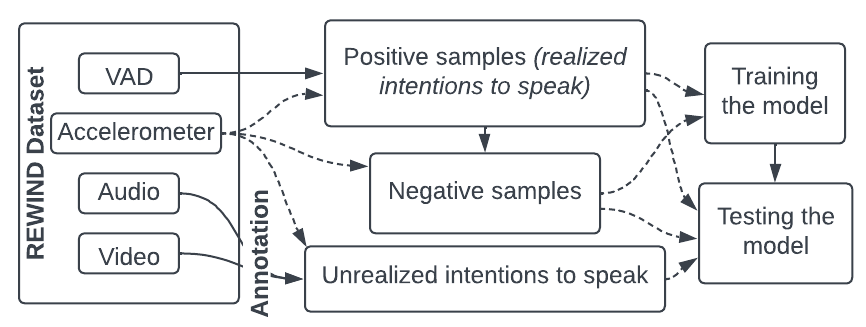
\includegraphics[width=0.6\columnwidth]{samples/INTS_overview (6).png}
  \vspace{-5mm}
  \caption{Overview of our approach. The dashed lines indicate the flow of only accelerometer data. 
% Note that the model is \emph{not} trained on the unrealized intentions to speak.
}  \vspace{-6mm}

  \label{fig:overview}
\end{figure}
% Using (heuristically) smoothed VAD, successful cases (windows) of intentions to speak are automatically extracted. These are used as positive samples for the model.
% Randomly selected windows without overlap with successful cases are extracted and used as negative samples for the model.
An overview of our experiments are shown in Figure \ref{fig:overview}. 
Developing systems that work outside of the lab in in-the-wild ecologically valid settings adds some additional constraints to our problem space. This includes exploiting a sensing setup that would maximise the detection of unrealized intentions and  whilst being respectful of privacy concerns. Building on the promising results of estimating speaking status with accelerometers \cite{raman2022conflab,rewinddata} we leverage the ubiquity of the conference ID badge commonly hung around the neck. The badge form-factor can be exploited with sensors such as a tri-axial accelerometer which is most likely to capture the fine grained breathing activities observed by Wlodarczak and Heldner \cite{wlodarczak2020breathing}, as well as other intention related behavioural modalities (e.g. leaning, gaze via head pose). 
% Given that the chatter of the social event is quite loud, participants may also tend to speak a bit louder, leading to possibly more exaggerated breath inhalations. 
Given the loud background chatter associated with busy networking events, we decided against using the audio since detecting subtle noises could be more challenging. There are also privacy concerns when recording private conversations \cite{raman2022conflab,MnM2021_underline}. Multi-modal analyses are left for future work. 
% 
% We aim to infer perceivable intentions to speak in a privacy-preserving and ubiquitous way. Since accelerometers capture a superposition of useful behavioural modalities for intentions to speak, we do this inference based on accelerometer data only. Examples of such features are body movement, posture shifts, possibly breath patterns. This final feature will likely not be captured in fine-grained detail, as a wearable accelerometer such as a smart badge will not be as sensitive as a specialized breath sensor. This is a trade-off because specialized breath sensors are not feasible in-the-wild. 
% Towards this goal of inferring intentions to speak, 

Our experimental approach is summarized in Fig. \ref{fig:overview}; a model is trained on the accelerometer data of automatically extracted \emph{realized} intentions to speak (Sec. \ref{sec:training}). These positive samples are automatically extracted from the voice activity detection (VAD) as explained in Sec. \ref{sec:vad}. The trained model is evaluated on the automatically generated realized and also manually annotated unrealized intentions to speak (Sec. \ref{sec:annot}). We present the results in Sec. \ref{sec:res}.
% A classifier is trained on the accelerometer data of realized intentions to speak (as positive samples) and randomly selected negative samples, such that there is no overlap with the positive samples. These positive samples are automatically extracted from the voice activity detection (VAD) as explained in section \ref{sec:vad}. The trained classification model is then evaluated on annotated cases of unrealized intentions to speak. These annotated cases are only used for evaluation and not for training due to the small amount of annotated cases. An overview of our method is shown in Figure \ref{fig:overview}.




% \begin{figure*}
%   \begin{tabular}{cc}
%      \begin{tabular}{l} 
%         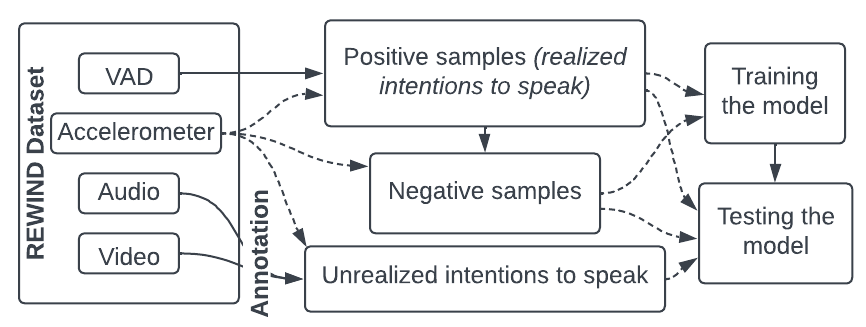
\includegraphics[width=0.48\textwidth]{samples/INTS_overview (6).png} 
%      \end{tabular}& 
%      \begin{tabular}{l} 
%         \includegraphics[width=0.4\textwidth]{samples/vad4.jpg}\\
%      \end{tabular}
%   \end{tabular}
%   \caption{\emph{Left:} A graphical overview of the case study; a model is trained on the accelerometer data of automatically extracted realized intentions to speak. This model is evaluated on annotated unrealized intentions to speak. Dashed lines indicate the flow of only accelerometer data. Note that the model is \emph{not} trained on the unrealized intentions to speak. \emph{Right:} Visualization of the VAD processing; short pauses are smoothed, short turns are ignored and a window of length \emph{x} before speech is used as a positive sample. The top image represents the raw voice activation. The bottom image represents the corresponding processed VAD.}
%   \label{fig:overview_and_vad}
% \end{figure*}



% \subsection{Exploratory Study of unrealised Intentions to Speak [merge with next]}
% \textbf{[Sketch: JORD]}
% Tried to become self-aware of cues that we think (can) indicate intentions to speak + dug in literature for cues, and listed all these cues
% => first word/syllable of utterance
% => hand raise
% => gaze patterns
% => deep breath to start speaking
% => mouth patterns (1. as proxy for breath patterns, 2. bite/compress/lick lip)
% => posture shifts
% => indirect; (attempt at) refusal to yield turn (talk louder / more fillers)
% => general body movement / motion distribution (Hayley had a nice graph for this)

% Looked at the REWIND dataset, looking for cues that (might) indicate an intention to speak
% => differentiate intentions to start speaking and intentions to continue speaking
% => audible mouth-opening patterns (lip/tongue click/smack)
% => lean towards other peoples ear in the presence of outside noise (essentially a posture shift, but a specific one)
% => throat clears

% We have a hunch that humans unconsiously are very good at inferring intentions to speak (e.g. based on gaze behaviour). Tried to explicitly look for them in private/personal social situations (drink with friends). => audible mouth-opening patterns (e.g. person A has an intention to speak, opens their mouth and by doing so smacks their lips. Then everybody looks at A expecting them to start speaking, and then A starts speaking) 

\subsection{Experimental Data}
For this case study, we used the REWIND dataset \cite{laughterquiros2023} which will soon be shared \cite{rewinddata}. The REWIND dataset contains audio, video, and wearable accelerometer data of an indoor professional networking event with around 100 attendees who stood and were free to mingle as they pleased. Video data is recorded by elevated side-view cameras, as shown in Fig. \ref{fig:teaser} (c). The event offered a mixed consent model where participants could choose whether to wear an accelerometer around their neck (like a conference ID badge), a wireless microphone attached to the face via specialised tape used for theatre productions, and appear under the cameras. A 10-minute segment (1:00:00 - 1:10:00) of the data is used for the exploratory study and annotations. In this interval, 13 participants had audio, video, and accelerometer data. Ethical approval from the university ethics board was granted.


\subsection{Labelling Unrealized Intentions to Speak}
\label{sec:annot}
To assess the quality of the model on unrealized intentions to speak, a sample of unrealized intentions to speak is needed. Before labelling the data, an initial exploratory study of unrealized intentions to speak was done. This involved critically examining our own behaviour in cases of intentions to speak and that of others. Finally, the data was observed to find cues that indicate intentions to speak. 

% From this observation, we found an important conceptual distinction between intentions to start speaking and intentions to continue speaking. Another important finding was that mouth-opening patterns through lip or tongue smacks were audible in some cases. Due to the loud background chatter, we found that people sometimes lean in or shift posture towards someone's ear when they want to say something. Lastly, throat clearing seemed also to indicate an intention to speak.

The most important finding from this exploratory study was that mouth-opening patterns through lip or tongue smacks were audible in some cases. To the best of our knowledge, no literature associates these audible mouth-opening patterns with intentions to speak. We claim that we should! Another finding from this exploratory study was that due the loud background chatter, we found that people sometimes lean in or shift posture towards someone's ear when they want to say something. Furthermore, throat clearing seemed also to indicate an intention to speak. Lastly, we found an important conceptual distinction between intentions to start speaking and intentions to continue speaking; in the first case, the person is not yet speaking and attempts to take the turn, whereas in the latter, the person is already speaking and attempts to \emph{keep} the turn. 

% After the exploratory study, samples of unrealized intentions to speak are generated by annotating a 10-minute segment (1:00:00 - 1:10:00) of the data. In this interval, 13 participants who had audio, video, and accelerometer data.
% were annotated A segment of 10 minutes was chosen because more would not be feasible given the time and resource limitations of this project, and this 10-minute window would need to be multiplied by the number of relevant participants (13, after removing the participants not in view of any camera) in order to get the total annotated time. 
% The segment was chosen to be 1:00:00 until 1:10:00 where participants were mingling. 
% This is somewhat arbitrary, but it does fulfil the requirement that the participants can move freely and talk to whom they want and about any topic they desire (e.g. the participants are not collectively listening to a public speaker and are not asked to play a conversational game with assigned conversation partners). 
% Taking the intersection of participants with a microphone and an accelerometer, and removing participants that are not in view of any camera in the segment, and with fully working audio date, 13 relevant participants remain. 
% There was one person with audio issues, so in the end there were 13 participants of interest.

% Given this segment, one (native Dutch) of the authors of this work performed the annotation 
After the exploratory study, during the 10-minute segment, start and end times of perceived unrealized intentions to speak were labelled manually.
An important consideration is that these are annotations of \emph{perceived} unrealized intentions to speak; when the annotator deemed it more likely than not the case that a person wanted to say something but did not (get the chance to), the segment is annotated.  The end of an annotated unrealized intention is labelled based on when the person does not speak when the annotator would expect them to speak and also when they do not give any signals anymore that they have an intention. 
% Annotating a perceived unrealized intention to speak is clearly a less well-defined task than annotating e.g. an apple in an image.
This highlights the inherent uncertainty in these annotations and the higher dependence on gut feeling of the annotator. 

Annotations were performed by one of the co-authors
using ELAN \cite{elan} using audio-visual data coming from the microphone and corresponding camera of a given subject. 
The annotator listened to one participant at a time while looking at them through the camera in which they are best visible. 
When the annotator perceived a (likely) unrealized intention to speak, this segment was annotated. This is primarily based on human intuition, whilst baring in mind the cues associated with (both realized and unrealized) intentions to speak that were identified in the literature survey and the exploratory study.

Following the findings of the exploratory study where we had identified two categories of unrealized intentions; starting and continuing to speak. We report from the chosen experimental data the number of observed unique individuals, samples, and mean, and standard deviation of the interval lengths respectively: intentions to take the turn (\textbf{UnrealStart}: $10,22,1.98\pm0.89s$ ) and intentions to continue speaking (\textbf{UnrealCont}: $7,17,2.46\pm0.97s$). 
% After the annotations were finished, they were processed to a usable format in Python using the pympi library \cite{pympi-1.70} and will be shared.
It is important to note that small sample size. This suggested that we would not be able to train a model from scratch with reasonable accuracy and that an alternative training approach was needed.


\subsection{Training Intentions to Speak}
\label{sec:training}
% To scrutinize the potential utility of an accelerometer for detecting speech intention, 
Four models were trained with varying window lengths spanning $1$-$4$s with $10$ epochs under $3$-fold cross-validation. To minimise variation in the model performance to discern differences between the different experiments, leave-person-out cross validation was not used. With so few test samples, we decided to train models for just \emph{realized} intentions to speak and test on the samples identified in Sec. \ref{sec:annot}. These models were evaluated using the ROC AUC across 5 experiments using different types of positive test samples \footnote{code and data shared at \url{https://github.com/llt-warlock/unrealizedIntention}};\textbf{1. All}: realized and unrealized intentions, 
\textbf{2. Realized}, 
\textbf{3. Unrealized}, 
 \textbf{4. UnrealStart}: unrealized intentions to start speaking, and \textbf{5. UnrealCont}: unrealized intentions to continue speaking.

 Adapting the implementation of Vargas et al. \cite{laughterquiros2023}, the structural architecture of our models comprises multiple residual neural networks embedded within convolutional neural networks. Non-overlapping training samples from individual accelerometer data were sampled from the mingling time outside of our chosen 10 minute segment and within the 10 minute segment for the test data.  This procedure was repeated 100 times. 

\subsubsection{Voice Activity Pre-processing}
\label{sec:vad}
For each speaker, we process the provided automatically detected voice activity generated by REWIND which computes voice activity by applying the following to each audio signal; loudness normalization, denoising, and Speaker diarization via NVIDIA NeMo \cite{kuchaiev2019nemo}. This was then processed to remove extremely short turns (<1.5s) that are likely to be back-channels and short pauses (<1.5s) between speaking. The threshold of 1.5s was determined empirically. 
% address two specific challenges. The first challenge pertains to microphone activation caused by short backchannels, while the second challenge involves microphone deactivation when a speaker momentarily pauses but maintains the turn. These issues are effectively resolved through preprocessing techniques. 
% In the Voice Activation Files (VAD) methodology, pauses shorter than 1.5 seconds are assigned a value of 1, indicating activation. Similarly, turns shorter than 1.5 seconds are assigned a value of 0, indicating deactivation. 
% It is important to note that these numerical thresholds have been optimized through a manual empirical process. 
% The smoothing procedure is illustrated in the left part of of Fig. \ref{fig:vad}. 

% \begin{figure}[tb]
%   \includegraphics[width=0.35\textwidth]{samples/vad5.jpg}
%   \vspace{-5mm}
%   \caption{Visualization of a smoothed voice activity signal; see Sec. \ref{sec:vad} for details. All positive samples are located just before the onset of speech (red) with duration \emph{x}. y axis: presence(1) or absence (0) of voice activity. }
%     \vspace{-5mm}
%   \label{fig:vad}
% \end{figure}



% \begin{figure}[hb]
%   \includegraphics[width=0.5\textwidth]{samples/vad2.jpg}
%   \caption{Visualization of the VAD processing; pauses are smoothed, short turns are ignored and a window of length \emph{x} before speech is used as a positive sample.}
%   \label{fig:vad}
% \end{figure}

% \begin{figure}[hb]
%   \includegraphics[width=0.43\textwidth]{samples/vad4.jpg}
%   \caption{Visualization of the VAD processing; short pauses are smoothed, short turns are ignored and a window of length \emph{x} before speech is used as a positive sample. The top image represents the raw voice activation. The bottom image represents the corresponding processed VAD.}
%   \label{fig:vad}
% \end{figure}

\subsubsection{Positive Sample Set Generation}
Since there were so few sample identified of unrealised intentions, we needed to leverage the large number of positive samples that existed in the dataset. We hypothesized that the unrealized intentions might have similar characteristics to the realized intentions, though findings by Wlodarczak and Heldner suggest that humans do adapt their behaviour some time before the next speaker when they can see that they will not get to speak\cite{wlodarczak2020breathing}. 

\begin{figure}[tb]
  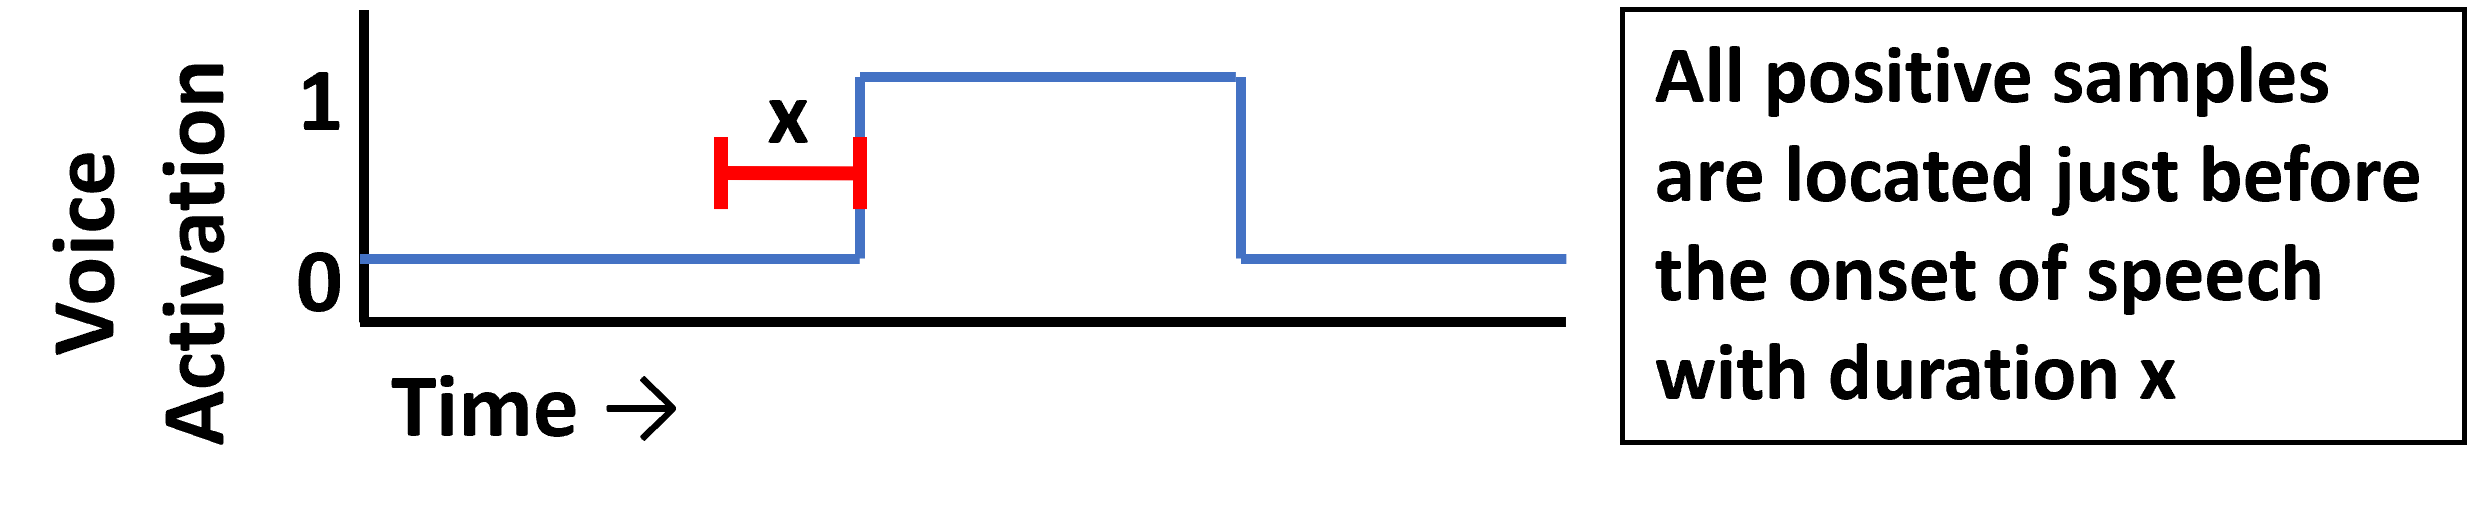
\includegraphics[width=0.6\columnwidth]{samples/vad10.png}
  \vspace{-4mm}
  \caption{Positive sample generation; X is varied from 1-4s.}
    \vspace{-2mm}
  \label{fig:vad}
\end{figure}
Positive realized intention samples were selected as the time windows prior to the activation of voice activity (interval X in Fig.\ref{fig:vad}). As the window length increases from 1 up to 4 seconds, the number of positive samples decrease due to a higher chance of overlapping with speaking segments. The length of time for the annotated positive unrealized intention also samples varies (as mentioned in Sec. \ref{sec:annot}). Since there were so few samples, we decided to use them all at test time irrespective of the window length. In all experiments, we aligned the end of the sample with the annotated end time of the positive unrealized intention sample and then computed back in time for the corresponding window length. The number of positive samples for training and test are shown in Tab. \ref{tab:experiment}.
% : the number of positive samples of "realized intention" varies under different time windows, while the number of positive samples of "unrealized intention" remains the same.  





% \begin{table}[H]
% \centering
% \scalebox{0.7}{
% \begin{tabular}{|l|c|c|c|c|}
% \hline
% \textbf{Experiment} & \textbf{\makecell[c]{realized \\ intention}} & \textbf{\makecell[c]{unrealized \\ intention (start)}} & \textbf{\makecell[c]{unrealized \\ intention \\ (continue)}} & \textbf{\makecell[c]{number of \\ positive \\ samples}} \\ \hline
% \textbf{Training} & $\checkmark$ &  & & 2894 \\  \hline
% \textbf{All} & $\checkmark$ & $\checkmark$  & $\checkmark$ & 327 \\  \hline
% \textbf{Realized}  & $\checkmark$  &  &  & 286\\ \hline
% \textbf{Unrealized}  &   & $\checkmark$ & $\checkmark$  & 41 \\ \hline
% \textbf{UnrealStart}  &   & $\checkmark$ &  & 22 \\ \hline
% \textbf{UnrealCont}  &   &  & $\checkmark$  & 19 \\ \hline

% \end{tabular}
% }
% \caption{Test dataset of experiments}
% \label{tab:experiment}
% \end{table}

\begin{table}[tb]
  \centering
  % \scalebox{0.4}
  
  \begin{tabular}{|c|c|c|c|c|} \hline 
      \multicolumn{2}{|c|}{} & \textbf{Realized}& \textbf{\makecell[c]{Unrealized\\Start}}&\textbf{\makecell[c]{Unrealized\\Continue}} \\ \hline

    \multicolumn{2}{|c|}{Train} & \cellcolor{cyan!15}2567 / 2053 / 1689 / 1487 &\cellcolor{red!5} unused &\cellcolor{red!5} unused \\ \hline

  { \parbox[t]{2mm}{\multirow{5}{*}{\rotatebox[origin=c]{90}{Experiment}}}}  & 1 &\multicolumn{3}{c|}{\cellcolor{cyan!15}327 / 268 / 239 / 217 }  \\ \cline{2-5}
    &2 & \cellcolor{cyan!15}286 / 227 / 198 / 176 &\cellcolor{red!5}unused &\cellcolor{red!5} unused  \\ \cline{2-5}
    &3 & \cellcolor{red!5} unused &  \multicolumn{2}{c|}{\cellcolor{cyan!15}39/39/39/39}   \\ \cline{2-5}
    &4 & \cellcolor{red!5} unused & \cellcolor{cyan!15}22/22/22/22 & \cellcolor{red!5} unused \\ \cline{2-5}
    &5 & \cellcolor{red!5} unused  & \cellcolor{red!5} unused & \cellcolor{cyan!15}17/17/17/17    \\ \hline
  \end{tabular}
  \caption{Numbers of positive samples by type: row 1. training; row 2-6: test samples generated at 1s/2s/3s/4s window lengths. Experiments with the different types of training data that was used; 1. All: realized and unrealized intentions, 2. Realized, and 3. Unrealized, 4.
UnrealStart: unrealized intentions to start speaking, and 5. UnrealCont: unrealized intentions to continue speaking.}
  \vspace{-5mm}
  \label{tab:experiment}
\end{table}



\subsubsection{Negative Sample Set Generation}
\label{negative sample set}
% In addition to the predetermined positive samples of accelerometer data, which are accompanied by a time window interval immediately preceding the speaking state, the 
The negative samples for training were randomly sampled outside the period 1:00:00-1:10:00, where the length of the negative samples corresponds to the length of the positive samples (1-4s). Test samples were randomly sampled from the time interval of 1:00:00-1:10:00 taking care that they did not overlap with any of the positive samples (experiment 2). The negative test samples for experiments 3, 4, and 5 were sampled from this same segment and did not overlap with positive realized or unrealized intention samples. The negative samples generated for experiment 1 also included the negative samples of experiments 2 and 3. The ratio of positive to negative samples is always 1:20.

% the negative samples randomly sampled in Experiment 2 did not overlap with the time periods of the positive samples of realized intentions. The negative of experiments 3, 4, and 5 samples were randomly generated and did not overlap with the time period of corresponding positive samples (Table \ref{tab:experiment}) and realized intention samples. The negative samples generated in Experiment 1 were a combination of the negative samples from Experiments 2 and 3. The ratio of positive samples to negative samples is maintained at 1:20. 

\subsection{Results}
\label{sec:res}
% \subsubsection{Evaluation of the model}
% For all experiments, the trained models were used to analyze the classification quality on the test sets under four different time windows. This procedure was repeated 100 times
% to make the results more stable and 
% to get a reliable estimate of the means and standard deviations of the AUC. 
A comparison of all the results are shown in Fig. \ref{fig:all-result} where the mean and standard error were computed over all folds over 100 runs. We observe that \textbf{Realized} had above average performance with better performance for longer windows and that \textbf{All} performs worse but still mostly above average. \textbf{Unrealized} shows performance comparable to \textbf{Realized} for 1s and 2s windows. However \textbf{Unrealized} has poor performance at windows of 3s or 4s, which could suggest that the unrealized intentional behavior is different further before the unrealized intention or that the labelling of the end of the unrealized intention was too far away from the start. 

Finally, dividing up the data from \textbf{Unrealized}, we observe that \textbf{UnrealCont} has consistently worse performance while \textbf{UnrealStart} has surprisingly better performance than all other experiments for 1s and 2s windows. This suggests that Unrealized intentions to start speaking exhibit extremely clear non-verbal behaviors that align well with the behavior of realized intentions. The performance drop as the window size increases could suggest that annotation of the end of the \textbf{UnrealStart} cases are shorter. These shorter window lengths also align with clear behaviours related to the intention to speak such as leaning. 

We speculate that unrealized intentions to continue speaking have more subtle behaviour since the subjects did not need to coordinate a turn change. The comparable performance of \textbf{UnrealCont} at 1s suggests that distinguishing behaviours are short such as for breathing. Finally, the general decreasing trend of experiments 3-5 as the window size increases may be due to samples being more and more contaminated by voice activity behavior. 
% This provides evidence that intention to speak behavior is very different from speaking behaviour.



% According to the results, the models trained with 1s and 2s windows can identify some patterns of unrealized intentions to speak but perform worse as the window size increases. Since we kept all the samples as the window length grew, we speculate that this could be related to the test window being increasingly contaminated with moments of voice activity. 
% For unrealized intentions, the models perform better with a shorter time window size. Due to the method of how we generated positive samples for unrealized intentions, as the size of time window increased, these samples would contain invalid data, which might reduce the performance. We speculate that unrealized intentions tend to happen in a small period of time, increasing the time window size can include less informative data related to unrealized intentions. 

% For unrealized intentions, the mean AUC decreases as the time window increases. For the realized intentions, the mean AUC score first decreases before the 2-second window, and then increases and reaches to the highest of all the five experiments after 2 seconds. In the first two windows, the model performs the best at predicting the unrealized intentions to start speaking. 

\begin{figure}[tb]
  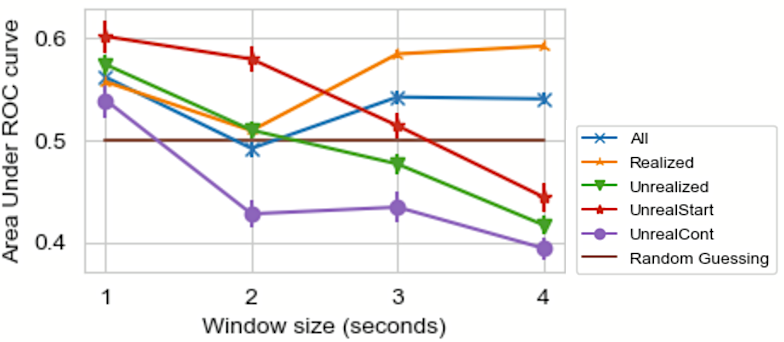
\includegraphics[width=0.5\columnwidth]{samples/result-all-2.png}
  \vspace{-5mm}
  \caption{ 
  Mean and standard deviation for all experiments.
}
\vspace{-5mm}
  \label{fig:all-result}
\end{figure}


% \begin{table}[H]
% \centering
% \scalebox{0.7}{
% \begin{tabular}{|l|l|l|l|l|}
% \hline
% \textbf{AUC scores}  &  \textbf{1 second}  & \textbf{2 seconds} & \textbf{3 seconds} & \textbf{4 seconds} \\ \hline
% \textbf{all intentions to speak} & 0.5618 (0.007)  & 0.4919 (0.008) & 0.5423 (0.007) & 0.5405 (0.006)\\ \hline
% \textbf{realized}  & 0.5573 (0.004) & 0.5093 (0.004)  & 0.5846 (0.004)  & 0.5923 (0.004) \\ \hline
% \textbf{unrealized} & 0.5742 (0.010) & 0.5098 (0.009) & 0.4766 (0.010) & 0.4168 (0.009)\\ \hline
% \textbf{unrealized (start)} & 0.6018 (0.016) & 0.5796(0.012) & 0.5142 (0.012) & 0.4442 (0.014) \\ \hline
% \textbf{unrealized (continue)} & 0.5393 (0.018) & 0.4276 (0.013) & 0.4342 (0.015) & 0.3939 (0.011)\\ \hline

% \end{tabular}
% }
% \caption{Mean (standard deviation) of ROC AUC scores for the evaluation on realized intentions to speak, unrealized intentions to start speaking and unrealized intentions to continue speaking.}
% \label{tab:auc_results}
% \end{table}


% \subsubsection{Comparison to random guessing}
% To compare the model's performance to random guessing, t-tests were done. The null hypothesis is $H_0$: ``The model performs the same as or worse than random guessing". The alternative hypothesis is $H_1$: ``The model performs better than random guessing". For each model evaluation configuration, as in table \ref{tab:auc_results}, a mean and a standard deviation of the AUC scores exist. Random guessing has a mean AUC of 0.5. In addition, we assume that the standard deviations of the AUC for random guessing are the same as the standard deviations in table \ref{tab:auc_results}. One-sided t-tests are done to see if the model performs better than random guessing. The p-values of the t-tests are given in table \ref{tab:ttest}. The values are compared to the (conservative) threshold of 0.001. 

% the comparison results are indicated with color in the table. Green color means that the result is significant and the null hypothesis can be rejected, meaning that the model performed better than random guessing. Red color means that there is not enough evidence to reject the null hypothesis.

% \begin{table}[h]
% \centering
% \scalebox{0.7}{
% \begin{tabular}{|l|l|l|l|l|}
% \hline
% \textbf{p-values}  & \textbf{1 second}  & \textbf{2 seconds} & \textbf{3 seconds} & \textbf{4 seconds} \\ \hline
% \textbf{all intentions to speak} & 6.545e-185 & 4.287e-138 & 1.0000 & 1.0000\\ \hline
% \textbf{realized}  & 4.889e-77 & 1.099e-29  & 0.2402  & 0.9996 \\ \hline
% \textbf{unrealized} & 1.575e-88 & 1.166e-98 & 1.0000 & 1.0000\\ \hline
% \textbf{unrealized (start)} & 3.130e-33 & 3.069e-138 & 1.293e-53 & 1.725e-125 \\ \hline
% \textbf{unrealized (continue)} & 1.241e-115 & 5.528e-75 & 0.9974 & 1.0000\\ \hline
% \end{tabular}
% }
% \caption{P-values for the t-tests comparing the model performance to random guessing. }
% \label{tab:ttest}
% \end{table}

% \begin{table}[h]
% \centering
% \scalebox{0.7}{
% \begin{tabular}{|l|l|l|l|l|}
% \hline
% \textbf{p-values}  & \textbf{1 second}  & \textbf{2 seconds} & \textbf{3 seconds} & \textbf{4 seconds} \\ \hline
% \textbf{all intentions to speak} & 2.099E-96 & 1.000 & 5.868E-82 & 6.081E-86\\ \hline
% \textbf{realized}  & 1.508E-144 & 8.249E-38  & 4.206E-135  & 2.894E-135 \\ \hline
% \textbf{unrealized} & 3.244E-90 & 6.793E-19 & 1.000 & 1.000\\ \hline
% \textbf{unrealized (start)} & 1.082E-82 & 6.732E-83 & 6.923E-20 & 1.000 \\ \hline
% \textbf{unrealized (continue)} & 4.442E-40 & 1.000 & 1.000 & 1.000\\ \hline
% \end{tabular}
% }
% \caption{P-values for the t-tests comparing the model performance to random guessing. }
% \label{tab:ttest}
% \end{table}


% \subsubsection{Linear regression through AUC scores}
% To explore the trends of increasing the size of the time window statistically, linear regression is applied. The slopes found by linear regression through the results of each experiment are presented in Table \ref{tab:regress}. Additionally, the $R^2$ measure (coefficient of determination) is presented. This measure indicates how well the regression model fits the data.

% \begin{table}[h]
% \centering
% \scalebox{0.7}{
% \begin{tabular}{|l|l|l|}
% \hline
%                         & \textbf{Slope} & \textbf{$R^2$} \\ \hline
% \textbf{All intentions to speak} & -0.0281 & 0.927 \\ \hline
% \textbf{Successful}              & -0.0253 & 0.750 \\ \hline
% \textbf{Unsuccessful}            & -0.0309 & 0.711 \\ \hline
% \textbf{Unsuccessful (Start)}    & 0.0063 & 0.0658\\ \hline
% \textbf{Unsuccessful (Continue)} & -0.0473 & 0.967 \\ \hline
% \end{tabular}
% }
% \caption{Slopes and $R^2$ values for linear regressions through the results. $R^2$ close to 0 indicates a bad fit and close to 1 indicates a good fit.}
% \label{tab:regress}
% \end{table}

% \subsubsection{Difference between intention to start and continue speaking}
% For every window size, a Welch's t-test\footnote{Does not necessarily assume equal variance for the two samples.} is performed, comparing the data. The null hypothesis is $H_0$: ``The samples have the same mean". The alternative hypothesis is $H_1$: ``The samples have different means".
% The p-values for a window size of 1, 2, 3, and 4 seconds are 1.979e-89, 4.843e-93, 5.594e-62, and 3.325e-175 respectively. Hence, for each considered window size, the null hypothesis can be rejected. 


\section{Summary and Open Challenges}
%unrealized intentions CAN be perceived and can be detected. But the semantic gap is larger. This leads to the issue of subjectivity.
%how often do unrealized intentions occur? How would learned representations handle these types of behaviors? What is the common pattern when unrealized intentions occur? probably the outcome constellation looks very different... or perhaps too varied to learn any regular patterns from?
%
We have proposed a reframing of intention estimation research to account for both realized and unrealized intentions to overcome the "intention by outcome" problem. We carried out a preliminary investigation showing that unrealized intentions can be labelled by an external observer. Our experiments using trained models demonstrate that realized and unrealized intentions are hard to disentangle which suggests potential opportunities to exploit transfer learning approaches. Beside this, many open questions remain:

\paragraph {Intention Detection vs. Segmentation}
Our case study presented a simple first step where we used a window based approach to decide if it contains an intention to speak or not. This requires us to know the length of an overt intention behaviour beforehand. There is likely to be a preference for finer grained annotations where we can observe the precise time when an intentional behaviour starts and also ends. Performing the labelling for the segmentation task when there are realized intentions is fine; one chooses the moment within a window of time when the start of an overt intentional behaviour is observed. But how do we label the start \emph{and end} of a intention that is never realized? Was the choice we made in the case study correct to rely on intuition to find the end of the intention rather than e.g. selecting the end of the first overt behaviour?

\paragraph {Associating Intentions with Outcomes}
For the case of realized intentions, finding the associated moment where the overt intention starts to occur follows prior work. However, even if we can use our gut instincts to identify an unrealized intention, was it right that the unrealized intention needs to occur shortly after the intention? What if it happens much later on? Or for more complex intentions where the outcome might be far in the future, how do we associate intentions with outcomes if there are long temporal connections? How long should a system wait before declaring an intention to be (un)realized? 
\paragraph {Subjectivity}
Our case study used one annotator. Without an associated outcome, unrealized intention labelling requires an observer to fill the gap between the observed cues and the perceived intent using on their own life experiences. For example, for the example initially given in Figure \ref{fig:teaser} (d), we may have a multiple equally plausible narratives of intention as perceived by different annotators (see Figure \ref{fig:multiintent}). 
\begin{figure}
    \centering
    \includegraphics[width=\linewidth]{samples/MultipleNarrativesIntent.png}
    \caption{What is the intent of subject E? If we were to ask multiple independent annotators, they may come up with multiple different intentions with all equally plausible explanations. Probably every annotator has a valid perception. It is not clear how we should set up a learning problem based on multiple equally valid but potentially conflicting narratives.}
    \label{fig:multiintent}
\end{figure}
Usually subjectivity is treated as noise but is there not a validity to any perception as long it is explained by observed cues? If so, how can we train models to account for this? What if all these equally valid perceptions do not agree despite each having very valid explanations?

\paragraph {Annotator Context}
As argued by Dudzik et al., a lack of systematic treatment of annotator context could be limiting system performance for affect perceptions\cite{dudzik2019context} and could apply to other labelling tasks. Thus far, the relevance of annotator context in annotation tasks is largely ignored. The Perspectivist Data Manifesto proposed by researchers in the Natural Language Processing Community could provide some useful insights \cite{Cabitza2023}. If integrated into the labelling task, this could allow systems to be designed to take only certain types of biases or perspectives into model training based on a careful selection of the context of annotators. Being able to manipulate the type of perspective that an estimated intention should originate from may also provide opportunities to get closer to the intent of the actual subject in question. Could the perspective of annotators that are closer to that of the subject make them better estimators of the true intention of the subject?

\paragraph {Situation Context}
The case study only addressed one type of intention. However, if we need to automatically infer multiple intentions, the context plays a significant role in how people perceive other people's overt intentions \cite{Alhasan2023}. As can be observed in Figure \ref{fig:multiintent}, when multiple plausible narratives of intent can exist for the same stimulus, the way to differentiate them comes from the explanation that accompanies an intent label. The explanations are interpretations based on an understanding of the context. In the illustrated example, they relate to social aspects such as who is currently socially involved with whom and temporal aspects such what is happening in the conversation(s) of interest. Detecting the social context is also a challenging problem as a model that plausibly defines conversational interaction as a fine time scale remains and open and challenging problem \cite{raman2019towards,10.1109/FG52635.2021.9667061,tan2022conversation,10.1145/3462244.3479963}





% \paragraph {Localizing Intentions and Time} Temporal granularity was lost with our detection based model in the case study. Our experiments show no consistent trend across the different window sizes. Using localization methods may improve performance. However, labelling the end time for an unrealized intention needs further investigation; 

% \subsection{Linking Proximal and Distal Intentions}
% The case study focused on a relatively short term intention. How does the problem change if more complex intentions are considered? e.g. intentions to join, leave a conversation, or start a conversation.

\paragraph {Multimodality}
Labelling the unrealized intentions required multimodal stimuli, although audio was the primary modality used. Further work is necessary to understand the interplay between different modalities and how they can be indicative of different types of intention. 
% Multi-modal approaches that have worked well with realized intention estimation should be investigated for unrealized intent. 

% \subsection{Relating True with Externally Perceived Intention}
% While there are scaling benefits to the third-party observer approach, we cannot deny the importance of the true intent of a user. There may be opportunities here to exploit third-party labels for personalization.

\paragraph {Potential for Societal Benefit} 
Some examples of how we could use intention estimation to reduce unwanted bias in issues of gender bias in teams or racism in criminal cases was discussed in the introduction. However, simply making estimates is not enough. How should a system respond to and act upon automated perceptions of realized and unrealized intentions? The matter may need to be handled extremely carefully for applications that counter discrimination and exclusion, especially when making an incorrect inference could be extremely damaging. Finally, the potential benefits of using intention estimation systems to help highlight how certain perspectives might lead to particular biases in intention estimation needs further exploration.


%%
%% The acknowledgments section is defined using the "acks" environment
%% (and NOT an unnumbered section). This ensures the proper
%% identification of the section in the article metadata, and the
%% consistent spelling of the heading.
% \begin{acks}
%Thanks to Tiffany, Stephanie, and Catha for their helpful feedback. 
% \end{acks}

%%
%% The next two lines define the bibliography style to be used, and
%% the bibliography file.
\pagebreak
\bibliographystyle{ACM-Reference-Format}
\bibliography{samples/references}


%%
%% If your work has an appendix, this is the place to put it.
% \appendix

% \section{Research Methods}

% \subsection{Part One}



\end{document}
\endinput
%%
%% End of file `sample-sigconf.tex'.
